%!TEX TS-program = pdflatex
%!TEX root = tesi.tex
%!TEX encoding = UTF-8 Unicode

\chapter{Risultati Ottenuti}
\todo[inline]{sommario capitolo}
% descrizione architettura migliore e a chi ci siamo ispirati N.R.
\todo[inline]
{
  Preambolo sulla accuratezza dei modelli creati
  Problema dell'AE perché non fornisce accuratezza, come parametro di valutazione si è utilizzata la loss
  La loss non poteva essere usata come discrtiminatoe perché troppo poco sensibile all'errore di presenza-nonpreseena della colla
  Un altro criterio di valutazione era una verifica a mano della qualità della differenza conforme in out

  Descrivere architettura migliore
  Descrivere post-processing a valle
}

\clearpage
\section{Il nostro obbiettivo TODO}
In figura~\ref{fig:obbiettivo_in_out_diff} sono riportate tre immagini per chiarire in che modo gli \textit{autoencoder} sono stati sfruttati per classificare Conformi e Scarti.
La figura~\ref{fig:obbiettivo_in} illustra uno Scarto.
L'immagine riportata in figura~\ref{fig:obbiettivo_out} è quella che si vorrebbe ottenere dall'AE a partire dallo Scarto appena illustrato.
Notare come si vorrebbe che il pezzo fosse riprodotto il più fedelmente possibile, ma che l'informazione della colla venisse rimossa.
In questo modo sarebbe possibile effettuare una differenza $pixel$ per $pixel$ tra immagine in ingresso ed immagine in uscita (detta anche ricostruita) ottenendo così un risultato simile a quello in figura~\ref{fig:obbiettivo_diff}.

Nel caso migliore possibile la classificazione verrebbe effettuata verificando se nell'immagine differenza tutti i valori sono zero.
Ossia l'immagine in ingresso appartiene alla classe Conforme ed è stata ricostruito alla perfezione.
Dato che ci si aspetta che l'autoencoder non ricostruisca la colla nell'immagine in uscita, nell'immagine differenza ci sarà un'area di pixel con valori in assoluto maggiori di zero.

Non possiamo aspettarci che l'autoencoder abbia una precisione così alta, ingatti è molto più probaile che l''immaine ricostruita sia soltatnot un''approssimzione dell'immagine in ingresso. \todo{fix here}
Si ricorda che molto probabilemte l'AE rimuoverà tutte quelle caratteristiche particolari di un pezzo (graffi, macchie, \dots )



Quindi la classificazione è divisa in due parti: prima l'immagine viene passata dell'autoencoder; poi viene effettuato del post-processing.

\begin{figure}[ht] % TODO
  \begin{center}
    \begin{tabular}{ccc}

      \begin{subfigure}{.3\linewidth}
        \centering\includegraphics[width=\textwidth]{example-image}
        \caption{Immagine in ingresso}
        \label{fig:obbiettivo_in}
      \end{subfigure} &

      \begin{subfigure}{.3\linewidth}
        \centering\includegraphics[width=\textwidth]{example-image}
        \caption{Immagine ricostruita}
        \label{fig:obbiettivo_out}
      \end{subfigure} &

      \begin{subfigure}{.3\linewidth}
        \centering\includegraphics[width=\textwidth]{example-image}
        \caption{Immagine differenza}
        \label{fig:obbiettivo_diff}
      \end{subfigure}

    \end{tabular}
    \caption{TODO in out diff}
    \label{fig:obbiettivo_in_out_diff}
  \end{center}
\end{figure}



\clearpage
\section{Metriche di valutazione}




\clearpage
\section{Architettura dell'autoencoder}

\begin{figure}[ht]
  \begin{center}
    \includegraphics[width=\textwidth]{example-image}
    \caption{TODO architettura della rete}
    \label{fig:ae16_arch}
  \end{center}
\end{figure}

\begin{figure}[ht]
  \begin{center}
    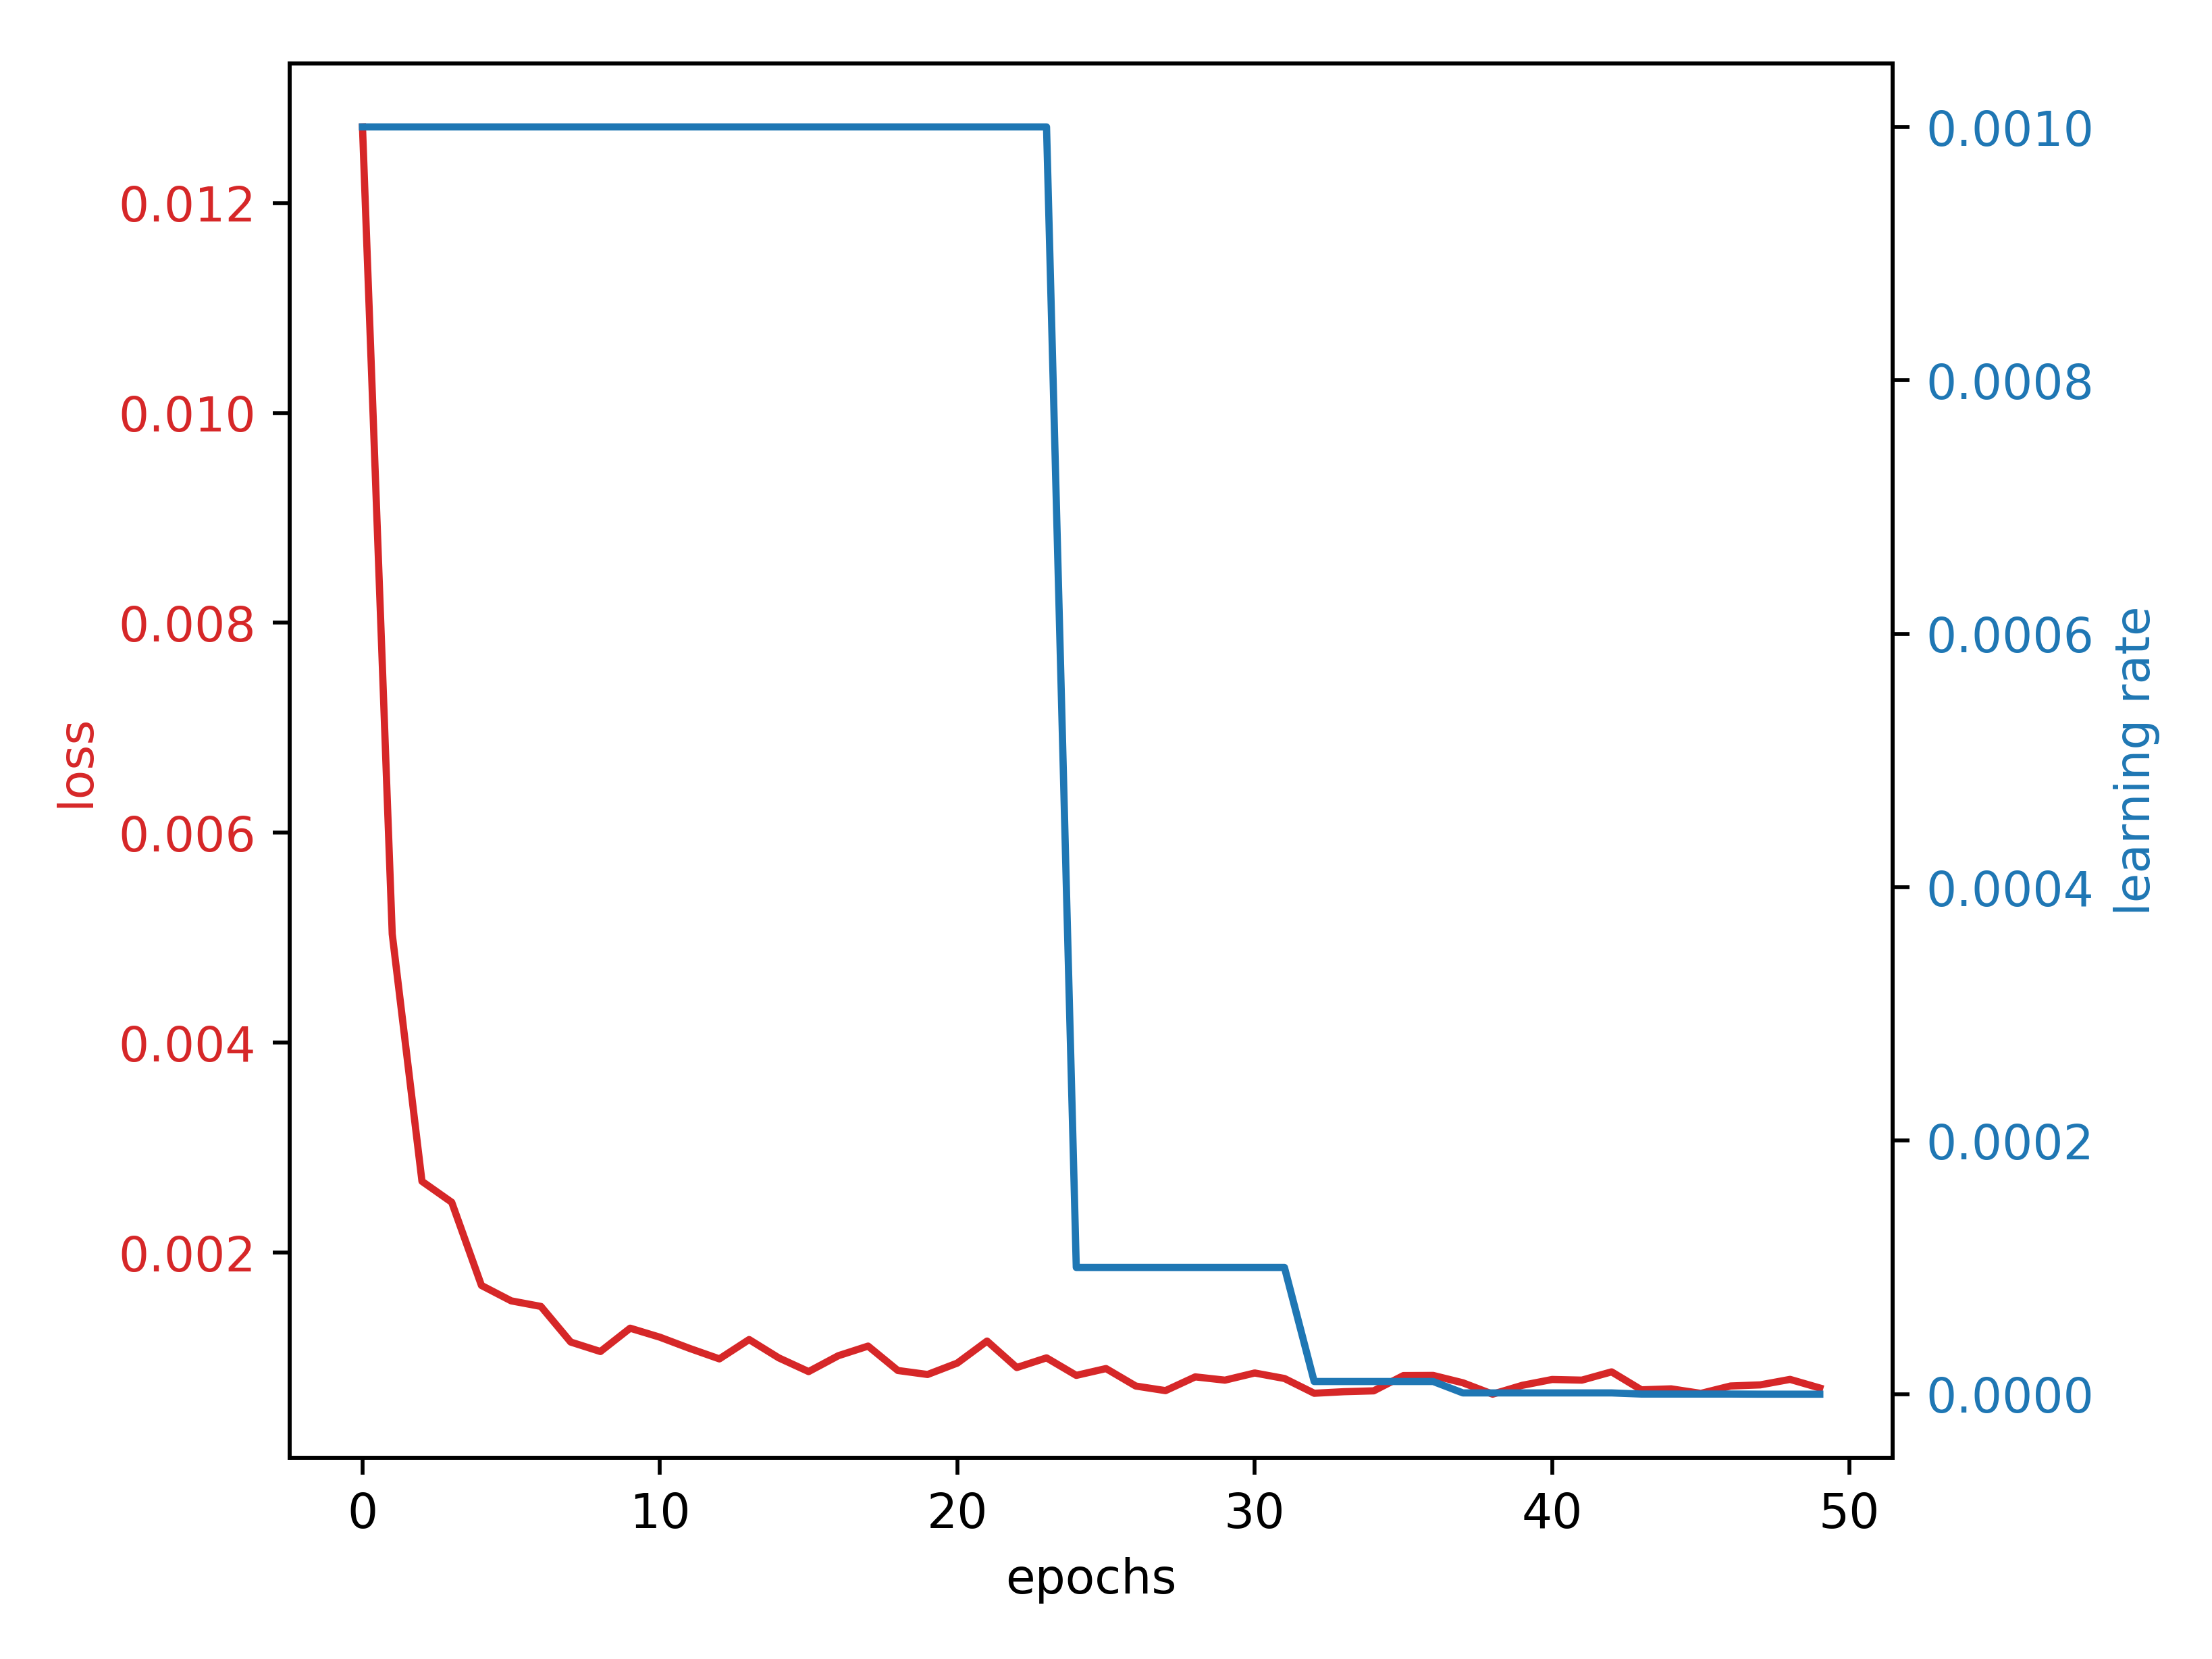
\includegraphics[width=0.8\textwidth]{loss_plot}
    \caption{TODO plot della loss}
    \label{fig:loss_plot}
  \end{center}
\end{figure}

\clearpage
\section{Post-Processing}
